\subsubsection{UC1 - Addestramento del sistema}%
\label{sssec:uc1}

\begin{figure}[h!]
  \begin{center}
    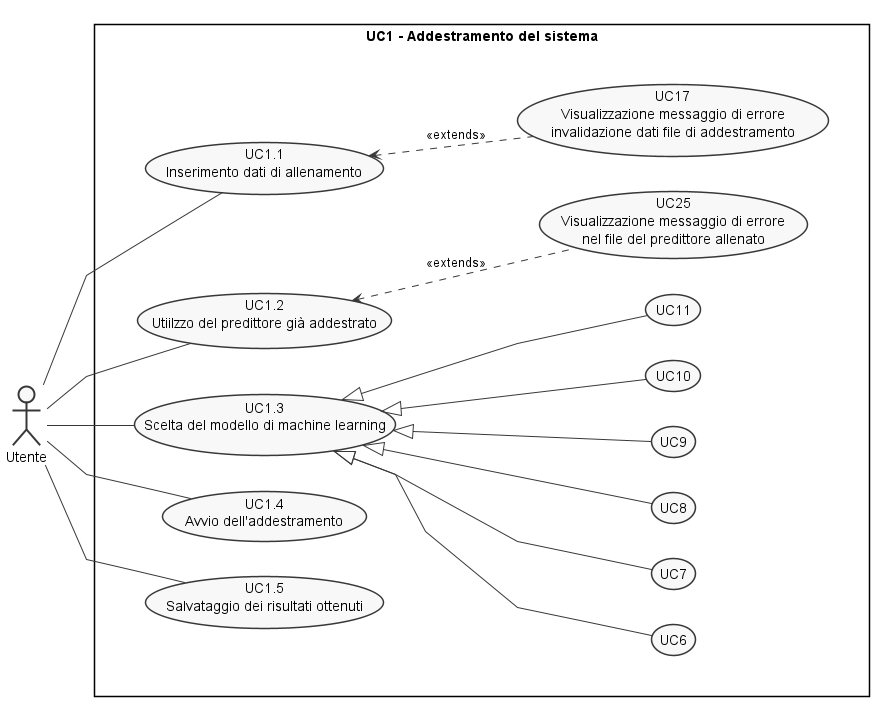
\includegraphics[width=14cm]{uc1.png}\\
    \caption{UC1 - Addestramento del sistema}%
    \label{fig:uc1}
  \end{center}
  \end{figure}

\begin{description}
  \item[Attore primario:] Utente amministratore.
  \item[Descrizione:] Per creare il file JSON contenente il predittore da dare al sistema di monitoraggio Grafana l'amministratore deve creare un file contenente i dati, scegliere il modello di machine learning da utilizzare e infine deve avviare l'addestramento.
  \item[Precondizione:] L'amministratore deve avere dei dati e sapere che modello utilizzare.
  \item[Scenario principale:]
  \begin{enumerate}
    \item L'amministratore inserisce i dati (UC1.1);
    \item L'amministratore utilizza un predittore già addestrato, se ne è in possesso (UC1.2);
    \item L'amministratore sceglie il modello di machine learning (UC1.3);
    \item L'amministratore avvia l'addestramento (UC1.4);
    \item L'amministratore crea un file contenente il predittore (UC1.5).
  \end{enumerate}
  \item[Postcondizione:] Si è ottenuto un file contente il predittore da dare a Grafana.
\end{description}

\paragraph{UC1.1 - Inserimento dati di allenamento}
\label{sssec:uc1.1}
\begin{description}
  \item[Attore primario:] Utente amministratore.
  \item[Descrizione:] L'amministratore inserisce i dati raccolti da un database in un file CSV.
  \item[Precondizione:] L'amministratore è in possesso di dati.
  \item[Scenario principale:]
  \begin{enumerate}
    \item L'amministratore carica i dati all'interno del file CSV;
    \item I dati vengono caricati nel sistema.
  \end{enumerate}
  \item[Postcondizione:] Il file CSV contiene i dati raccolti dall'amministratore.
  \item[Estensioni:] UC1.1 viene esteso nel caso d'uso UC8 con la visualizzazione del messaggio di errore quando viene fornito un file di addestramento non valido.
\end{description}

\paragraph{UC1.2 - Utilizzo del predittore già addestrato}
\label{sssec:uc1.2}
\begin{description}
  \item[Attore primario:] Utente amministratore.
  \item[Descrizione:] L'amministratore utilizza il file JSON contenente il predittore addestrato in un'applicazione esterna.
  \item[Precondizione:] L'amministratore ha a disposizione il predittore già allenato.
  \item[Scenario principale:] L'amministratore, qualora possieda un predittore precedentemente allenato, lo carica nel sistema.
  \item[Postcondizione:] L'amministratore ha a disposizione un predittore già addestrato.
  \item[Estensioni:] UC1.2 viene esteso nel caso d'uso UC16 con la visualizzazione del messaggio di errore quando si tenta di caricare un predittore in un formato non valido.
\end{description}

\newpage

\paragraph{UC1.3 - Scelta del modello di machine learning}%
\label{sssec:uc1.3}

\begin{figure}[h!]
  \begin{center}
    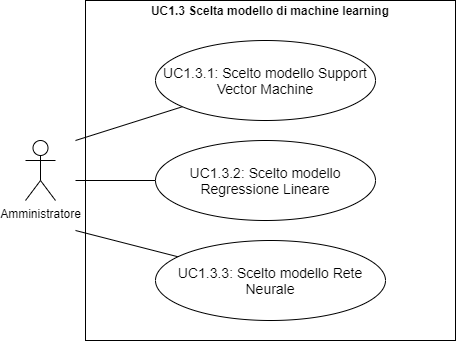
\includegraphics[width=10cm]{uc1.3.png}\\
    \caption{UC1.3 - Scelta del modello di machine learning}%
    \label{fig:uc1.3}
  \end{center}
\end{figure}

\begin{description}
  \item[Attore primario:] Utente amministratore.
  \item[Descrizione:] L'amministratore decide che tipo di machine learning utilizzare: SVM, RL o la Rete Neurale.
  \item[Precondizione:]
  \begin{enumerate}
    \item L'inserimento dei dati è avvenuto correttamente (UC1);
    \item L'amministratore ha a disposizione i tre modelli di machine learning.
  \end{enumerate}
  \item[Scenario principale:] L'amministratore, avente un file contenente i dati, decide che modello di machine learning utilizzare tra SVM, RL o la Rete Neurale.
  \item[Postcondizione:] L'amministratore ha scelto un modello di machine learning.
\end{description}

\subparagraph{UC1.3.1 - Scelto modello Support Vector Machine}%
\label{sssec:uc1.3.1}
\begin{description}
  \item[Attore primario]: Utente amministratore.
  \item[Descrizione]: L'amministratore ha scelto come modello la Support Vector Machine.
  \item[Precondizione:]
  \begin{enumerate}
    \item L'inserimento dei dati è avvenuto correttamente (UC1);
    \item L'amministratore ha a disposizione i tre modelli di machine learning.
  \end{enumerate}
  \item[Scenario principale:] L'amministratore ha selezionato SVM come algoritmo per svolgere l'addestramento.
  \item[Postcondizione]: L'amministratore ha scelto come modello la SVM.
\end{description}

\newpage

\subparagraph{UC1.3.2 - Scelto modello Regressione Lineare}%
\label{sssec:uc1.3.2}

\begin{figure}[h!]
  \begin{center}
    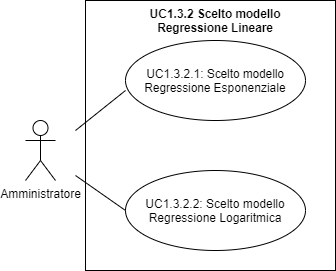
\includegraphics[width=10cm]{uc1.3.2.png}\\
    \caption{UC1.3.2 - Scelto modello Regressione Lineare}%
    \label{fig:uc1.3.2}
  \end{center}
  \end{figure}

\begin{description}
  \item[Attore primario]: Utente amministratore.
  \item[Descrizione]: L'amministratore ha scelto come modello la Regressione Lineare.
  \item[Precondizione:]
  \begin{enumerate}
    \item L'inserimento dei dati è avvenuto correttamente (UC1);
    \item L'amministratore ha a disposizione i tre modelli di machine learning.
  \end{enumerate}
  \item[Scenario principale:] L'amministratore ha selezionato la RL come algoritmo per svolgere l'addestramento.
  \item[Postcondizione]: L'amministratore ha scelto come modello la RL.
\end{description}

\subparagraph*{UC1.3.2.1 - Scelto modello Regressione Esponenziale}
\label{sssec:uc1.3.2.1}
\begin{description}
  \item[Attore primario]: Utente amministratore.
  \item[Descrizione]: L'amministratore ha scelto come modello la Regressione Esponenziale.
  \item[Precondizione:]
  \begin{enumerate}
    \item L'inserimento dei dati è avvenuto correttamente (UC1);
    \item L'amministratore ha a disposizione i tre modelli di machine learning.
  \end{enumerate}
  \item[Scenario principale:] L'amministratore ha selezionato la Regressione Esponenziale come algoritmo per svolgere l'addestramento.
  \item[Postcondizione]: L'amministratore ha scelto come modello la Regressione Esponenziale.
\end{description}

\subparagraph*{UC1.3.2.2 - Scelto modello Regressione Logaritmica}
\label{sssec:uc1.3.2.2}
\begin{description}
  \item[Attore primario]: Utente amministratore.
  \item[Descrizione]: L'amministratore ha scelto come modello la Regressione Logaritmica.
  \item[Precondizione:]
  \begin{enumerate}
    \item L'inserimento dei dati è avvenuto correttamente (UC1);
    \item L'amministratore ha a disposizione i tre modelli di machine learning.
  \end{enumerate}
  \item[Scenario principale:] L'amministratore ha selezionato la Regressione Logaritmica come algoritmo per svolgere l'addestramento.
  \item[Postcondizione]: L'amministratore ha scelto come modello la Regressione Logaritmica.
\end{description}

\subparagraph{UC1.3.3 - Scelto modello Rete Neurale}
\label{sssec:uc1.3.3}
\begin{description}
  \item[Attore primario]: Utente amministratore.
  \item[Descrizione]: L'amministratore ha scelto come modello la Rete Neurale.
  \item[Precondizione:]
  \begin{enumerate}
    \item L'inserimento dei dati è avvenuto correttamente (UC1);
    \item L'amministratore ha a disposizione i tre modelli di machine learning.
  \end{enumerate}
  \item[Scenario principale:] L'amministratore ha selezionato la Rete Neurale come algoritmo per svolgere l'addestramento.
  \item[Postcondizione]: L'amministratore ha scelto come modello la Rete Neurale.
\end{description}


\paragraph{UC1.4 - Avvio dell'addestramento}
\label{sssec:uc1.4}
\begin{description}
  \item[Attore primario:] Utente amministratore.
  \item[Descrizione:] L'amministratore utilizzando la libreria e i dati ottiene il predittore.
  \item[Precondizione:]
  \begin{enumerate}
    \item L'amministratore ha a disposizione il file contenente i dati (UC1);
    \item L'amministratore ha scelto un modello di machine learning.
  \end{enumerate}
  \item[Scenario principale:] Avendo a disposizione il file con i dati e avendo scelto un modello avviene l'addestramento.
  \item[Postcondizione:] Si è ottenuto il predittore.
\end{description}

\paragraph{UC1.5 - Salvataggio del risultati ottenuti}
\label{sssec:uc1.5}
\begin{description}
  \item[Attore primario:] Utente amministratore.
  \item[Descrizione:] I risultati ottenuti vengono salvati nel file JSON, riportando anche la tipologia di modello di machine learning utilizzato.
  \item[Precondizione:]
  \begin{enumerate}
    \item L'amministratore ha i dati ottenuti in precedenza;
    \item L'amministratore ha deciso che modello di machine learning  utilizzare.
  \end{enumerate}
  \item[Scenario principale:] Una volta ottenuti i risultati dall'addestramento, l'amministratore salva i dati e il modello utilizzato nel file JSON.
  \item[Postcondizione:] Il file contiene sia il predittore che il modello utilizzato.
\end{description}
